\documentclass[11pt]{standalone}
\usepackage{amssymb}
\usepackage{amsmath}
\usepackage[no-math]{fontspec}
\usepackage{unicode-math}
\usepackage{libertinus}
\usepackage{pgf,xcolor}
\usepackage{tikz}
\usetikzlibrary{arrows.meta, backgrounds, calc}
\usepackage{pgfplots}
\pgfplotsset{compat=newest}

\definecolor{my_darkgray}{HTML}{484949}
\definecolor{my_lightgray}{HTML}{F3F4F4}
\definecolor{my_darkblue}{HTML}{005A94}
\definecolor{my_lightblue}{HTML}{CCDEE9}
\definecolor{my_yellow}{HTML}{FFEC7F}
\definecolor{my_red}{HTML}{E60000}
\definecolor{my_orange}{HTML}{E87846}

\begin{document}
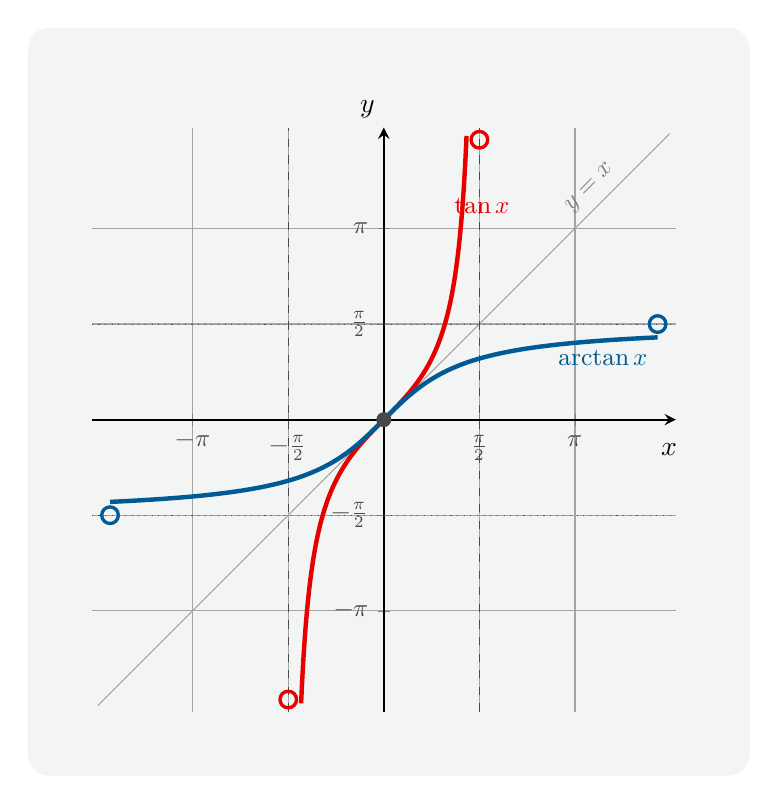
\begin{tikzpicture}[
    show background rectangle,
    background rectangle/.style={fill=my_lightgray, rounded corners=8pt},
    inner frame sep=0.8cm
]

% arctan(x): domain ℝ, range (-π/2, π/2) – open interval, horizontal asymptotes
% tan restricted to (-π/2, π/2): domain open interval, range ℝ, vertical asymptotes
% axis equal: preserves the mirror symmetry across y = x.
% Window clipped at ±4.5 to show both curves reaching their asymptotes visibly.
\begin{axis}[
    axis lines = center,
    xlabel = {$x$},
    ylabel = {$y$},
    xlabel style = {at={(axis cs:4.7,0)}, anchor=north, yshift=-5pt},
    ylabel style = {anchor=south east},
    grid = both,
    grid style = {line width=0.3pt, draw=my_darkgray!30},
    major grid style = {line width=0.5pt, draw=my_darkgray!50},
    axis equal,
    axis line style = {thick},
    xmin = -4.8, xmax = 4.8,
    ymin = -4.8, ymax = 4.8,
    xtick = {-3.14159, -1.5708, 0, 1.5708, 3.14159},
    xticklabels = {$-\pi$, $-\tfrac{\pi}{2}$, $0$, $\tfrac{\pi}{2}$, $\pi$},
    ytick = {-3.14159, -1.5708, 0, 1.5708, 3.14159},
    yticklabels = {$-\pi$, $-\tfrac{\pi}{2}$, $0$, $\tfrac{\pi}{2}$, $\pi$},
    yticklabel style = {font=\small, text=my_darkgray},
    xticklabel style = {font=\small, text=my_darkgray},
    width=9cm, height=9cm,
    clip=true,
]

% Diagonal y = x: mirror axis for the inverse relationship
\addplot[
    draw=my_darkgray!50,
    thin,
    domain=-4.7:4.7
]{ x };
\node[anchor=south, rotate=45, font=\small, text=my_darkgray!70]
    at (axis cs:3.6, 3.6) {$y = x$};

% Vertical asymptotes of tan at x = ±π/2
\foreach \xa in {-1.5708, 1.5708}{
    \addplot[draw=my_darkgray, dashed, thin]
        coordinates {(\xa,-4.8) (\xa,4.8)};
}

% Horizontal asymptotes of arctan at y = ±π/2 (open range boundary)
\foreach \ya in {-1.5708, 1.5708}{
    \addplot[draw=my_darkgray, dotted, thin, domain=-4.8:4.8]{ \ya };
}

% tan(x) restricted to (-π/2, π/2): open domain, restrict y guards the clip
\addplot[
    draw=my_red,
    samples=400,
    ultra thick,
    domain=-1.511:1.511,
    restrict y to domain=-4.8:4.8
]{ tan(deg(x)) };

\node[anchor=north west, font=\small, text=my_red]
    at (axis cs:1.0, 3.8) {$\tan x$};

% arctan(x) on all of ℝ; range stays strictly within (−π/2, π/2)
\addplot[
    draw=my_darkblue,
    samples=500,
    ultra thick,
    domain=-4.5:4.5
]{ atan(x) * pi / 180 };

\node[anchor=north east, font=\small, text=my_darkblue]
    at (axis cs:4.5, 1.3) {$\arctan x$};

% Mark the origin (0, 0), shared by both curves
\addplot[
    mark=*,
    mark size=2.5pt,
    only marks,
    draw=my_darkgray,
    fill=my_darkgray
] coordinates {(0, 0)};

% Open circles on tan curve at the asymptote boundary (clipped y ≈ ±4.6)
% indicating the domain is the open interval (-π/2, π/2)
\addplot[
    mark=o,
    mark size=3pt,
    only marks,
    draw=my_red,
    fill=my_lightgray,
    line width=1.2pt
] coordinates {(-1.5708, -4.6) (1.5708, 4.6)};

% Open circles on arctan curve at the asymptote boundary
% indicating the range is the open interval (-π/2, π/2)
\addplot[
    mark=o,
    mark size=3pt,
    only marks,
    draw=my_darkblue,
    fill=my_lightgray,
    line width=1.2pt
] coordinates {(-4.5, -1.5708) (4.5, 1.5708)};

\end{axis}
\end{tikzpicture}
\end{document}
